\documentclass[a4paper,10pt]{article}
\usepackage[utf8]{inputenc}
\usepackage{graphicx}
\usepackage{listings}
\usepackage{caption}
\usepackage{subcaption}
\usepackage{amsmath}
\usepackage{amsfonts}

\usepackage{listings}
\usepackage[usenames,dvipsnames]{color}
\usepackage{courier}
  
  % This is the color used for MATLAB comments below
\definecolor{MyDarkGreen}{rgb}{0.0,0.4,0.0}
\definecolor{MyPink}{rgb}{1.0,0.0,0.5}
\definecolor{gray}{rgb}{0.5,0.5,0.5}
\definecolor{MyRed}{rgb}{0.8,0.3,0.36}
% For faster processing, load Matlab syntax for listings
\lstloadlanguages{C}%
\lstset{ %
  language=C,						% the language of the code
  basicstyle=\footnotesize,         % the size of the fonts that are used for the code
  numbers=left,                   	% where to put the line-numbers
  numberstyle=\footnotesize,        % the size of the fonts that are used for the line-numbers
  stepnumber=1,                   	% the step between two line-numbers. If it's 1, each line 
                                  	% will be numbered
  numbersep=5pt,                  	% how far the line-numbers are from the code
  backgroundcolor=\color{white},    % choose the background color. You must add \usepackage{color}
  showspaces=false,               	% show spaces adding particular underscores
  showstringspaces=false,         	%	 underline spaces within strings
  showtabs=false,                 	% show tabs within strings adding particular underscores
  frame=single,                   	% adds a frame around the code
  rulecolor=\color{black},        	% if not set, the frame-color may be changed on line-breaks within not-black text (e.g. commens (green here))
  tabsize=2,                      	% sets default tabsize to 2 spaces
  captionpos=b,                   	% sets the caption-position to bottom
  breaklines=true,                	% sets automatic line breaking
  breakatwhitespace=true,        	% sets if automatic breaks should only happen at whitespace
  title=\lstname,                   % show the filename of files included with \lstinputlisting;
                                  	% also try caption instead of title
  numberstyle=\tiny\color{gray},    % line number style
  keywordstyle=\color{MyDarkGreen},        % keyword style
  commentstyle=\color{blue},       	% comment style
  stringstyle=\color{MyPink},       % string literal style
  escapeinside={\%*}{*)},           % if you want to add a comment within your code
  morekeywords={0,1,2,3,4,5,6,7,8,9}            	% if you want to add more keywords to the set
  }

\lstset{
emph={unsigned,char,double,int},emphstyle=\color{MyDarkGreen},
emph={[2]if,for,else,while,return},emphstyle={[2]\color{Red}},
emph={\#include},emphstyle=\color{MyDarkGreen},
emph={0,1,2,3,4,5,6,7,8,9},emphstyle=\color{MyPink}
}










% Title Page
\title{}
\author{}


\begin{document}

\begin{titlepage}
\begin{center}


\textsc{\LARGE Royal Institute of Technology}\\[1.5cm]


\includegraphics[width=0.3\textwidth]{kth_mathematics_rgb.jpg}\\[1cm]

\textsc{\Large Introduction to High-Performance Computing, DN2258 }  %\\ Instructor: Tobias Ryden , \emph{tryd@math.kth.se}}\\[0.5cm]

\hrulefill \\[0.4cm]
{ \huge \bfseries Final project, parallel search\\ Draft 2}\\[0.4cm]
\hrulefill \\[1.5cm]


Sindri Magnússon, sindrim@kth.se, 871209-7156 \\
Brynjar Smári Bjarnasson, bsbj@kth.se, 840824-4690 \\


\vfill
% Bottom of the page
{\large \today}

\end{center}
\end{titlepage}


%%%%%%%%%%%%%%%%%%%%%%%%%%%%%%%%%%%%%%%%%%%%%%%%%%%%%%%%%%%%%%%%%%%%%%%%%%%%%%%%
%%%%%%%%%%%%%%%%%%%%%%%%%%%%%%%%%%%%%%%%%%%%%%%%%%%%%%%%%%%%%%%%%%%%%%%%%%%%%%%%
%%%%%%%%%%%%%%%%%%%%%%%%%%%%%%%%%%%%%%%%%%%%%%%%%%%%%%%%%%%%%%%%%%%%%%%%%%%%%%%%
%%%%%%%%%%
%%%%%%%%%% Report statrs
%%%%%%%%%%
\cleardoublepage
\tableofcontents
\newpage

\section{Introduction}

In today's scientific environment the amount of data that is generated is increasing like never before.  
One consequence of these revolutionary times is the ability to process 
and work with this data in acceptable time.  
We plan to look further into one of the most important problem in the data universe which is searching.  


\subsection{The data}
To isolate the main problem and to be able to analyse the results in as direct way as possible we decided to use as simple data as we could think of.
Another benefit of a simple data set is the ability of creating a data with a large number of rows. 
The data set is a file containing in every line an id and a sequence of six uniform random integers on the interval $[0,9]$.  
All of the id's and all the sequences of random numbers have the same number of characters so the number of characters in each line is fixed.

Here below we see an example of the data with $10^7$ rows.
\lstinputlisting[language=C]{example_data.txt}  
The data we used for testing contains $10^{9}$ lines and each line has $17$ characters.  
Since a character is one byte
the file is $17 \times 10^9$ bytes ($17$ Gbyte).  We had some troubles working with this huge data
sets in MPI so we also ran some experiments where we reduced the data down to 2 Gbyte.

\section{Theoretical performance estimation}

Since each comparison in the search is independent we see that the problem of searching is actually 
embarrassingly parallel.  
However we need to read the data file from disk which is a sequential operation.  
So we can split the problem into two components the parallel part, the search,
and the sequential part, reading the data.
We expect to see a linear speed-up for the parallel part and
no speed-up for the sequential part.
%So if we only look at the searching part of the algorithm then we would expect a linear speedup.  

We now let $P$ be the time percent of the parallel  
part, so $1-P$ is the time percent of the sequential part.  
Then from Amdahl's law we expect the speedup on $N$ threads to be:
$$ S_N = \frac{1}{(1-P)+\frac{P}{N}}$$

\section{Implementation}
  
\subsection{OpenMP}

  
  The separation between the sequential and parallel part of the algorithm becomes very clear 
  for openmp. The reason for that is that first we read the data, sequentially, and then we
  split the actual search up on many threads with a OpenMP parallel for loop.  
  

\subsection{MPI whit MPI IO}
\label{sec:MPIO}

  We will use the following notation:
  \begin{align*}
    P &= \text{ number of processes} \\
    p &= \text{ current process}  \\
    L &= \text{ Nr of lines of data } 
  \end{align*}
  and $k:= L (\mod P)$, that is we have $n\in \mathbb{N}$ and integer $k$ with $0\leq k < P$
  such that $L = Pn+k$.  We make $n$ denote $\lfloor \frac{L}{P} \rfloor$.

  For the MPI implementation we use the MPI IO to make each process read part of the data file
  and then search it's part.  We split the data equally between the process but if
  P does not divide L evenly then we distribute the remaining elements to the last $k$ processes,
  that is processes $P-k,P-k+1,\cdots P-1$.
  
  The size of the data chunk on process $p$ will then be $n$ if $p<P-k$ and $n+1$ if $p\geq P-k$.
  That is the same as:
  \begin{align*}
    \lfloor \frac{L+p}{P}\rfloor  &= \lfloor \frac{Pn+k+p}{P}\rfloor  \\
                                  &= \lfloor n+\frac{k+p}{P}\rfloor   \\
                                  &=                                  
                                  \left\{
                                    \begin{array}{l l}
                                       n   & \quad \text{if $p<P-k$ }\\
                                       n+1 & \quad \text{if $p\geq P-k$}\\
                                     \end{array} \right.
  \end{align*}
  We split the data elements on the processes so that process $p$ 
  gets data elements 
  $p\left( n + \lfloor \frac{p}{P-k+1} \rfloor \right),
   p\left( n + \lfloor \frac{p}{P-k+1} \rfloor \right)+1, \cdots,
   (p+1)\left( n + \lfloor \frac{p+1}{P-k+1} \rfloor \right)-1
  $.
  That process $p$ such that $p<P-k$ takes the first $n$ elements
  after and with element $ p n $, process $p=P-k$ takes the first
  $n+1$ elements after and with $ p n $
  and process $p$ such that $p>P-k$ takes the first $n+1$ elements after and
  with element $ p n +1 $.
  Then each process searches in it's local data.

  One problem with this approach is that the sequential part of the algorithm, reading the data,
  might get some negative speed-up since the processes have battle each other 
  to be able to read there part of the data from the same file.  Our hope is that
  the MPI IO reading methods will take care of that problem, at least to some some extent.   
  
\section{MPI single read}
  Here we have the single root process reading the file and distributing the work on all processes. 
  The same calculations as in \ref{sec:MPIO} are used to figure out how many bytes to send to each process.  
  After reading the file, the root process broadcasts basic information about how many bytes are in the 
  file and how long each line is to all processes. Then we use MPI\_Scatterv to distribute the workload 
  to all processes. We hope that we can reduce the reading time compared to the \ref{sec:MPIO} method while 
  keeping linear speed-up on the searching part.



\section{Results}

\subsection{OpemMP}
 
 To examine the performance of our OpenMP implementation we 
 We ran our implementation of the OpenMP search algorithm $10$ times for each number
 of threads where the number of threads was $1,2,4,8,16,24$.
 In figure ~\ref{fig:openmp_load} and \ref{fig:openmp_search} we see the
 time it takes to read the data and the time it takes to search the data.
 The reading operation is a single thread operation and hence it should not differ for 
 different number of threads.  But that is not the case here, if we look at figure \ref{fig:openmp_load}
 we see that the average reading time is around $60$ seconds for all nr. of process except
 $1$ process.  The variation is also much more for one thread so there could be some 
 errors in the run for $1$ thread. 
 In figure~\ref{fig:openmp_speedup} we see the speed-up for the search. 
 The speed-up is very close to optimal which is not surprising since the search is embarrassingly
 parallel.
 In figure \ref{fig:openmp_amad1} we see the actual speed up of the code in comparison to Amdahls law.
 To calculate $P$, the time percent of the parallel part, in Amdahls law we look at the
 average reading time for one thread, $T_s$, and the average search time for one thread, $T_p$.
 Then we set $P=\frac{T_p}{T_p+T_s}$.  We can see from the figure that Amdahls law misses the speed-up 
 curve completely and the estimation we get from Amdahls law
 is much worse than the speed-up we actually get.
 But the average reading time for one thread was much higher than for when we had higher numbers of 
 threads.  It seemed more like the reading time was close to $60s$ and since the reading
 time does not depend on number of threads it seems reasonable to fix the reading time as $60s$.
 In figure \ref{fig:openmp_amad2} we see the total speed-up compared to Amdahls law
 when the reading time has been fixed to $60$ seconds.  Now our results agree with Amdals law
 which is not surprising since we got almost perfect speed up for the parallel part.

\begin{figure}[h!t]
        \centering
        \begin{subfigure}[b]{0.70\textwidth}
                \centering
                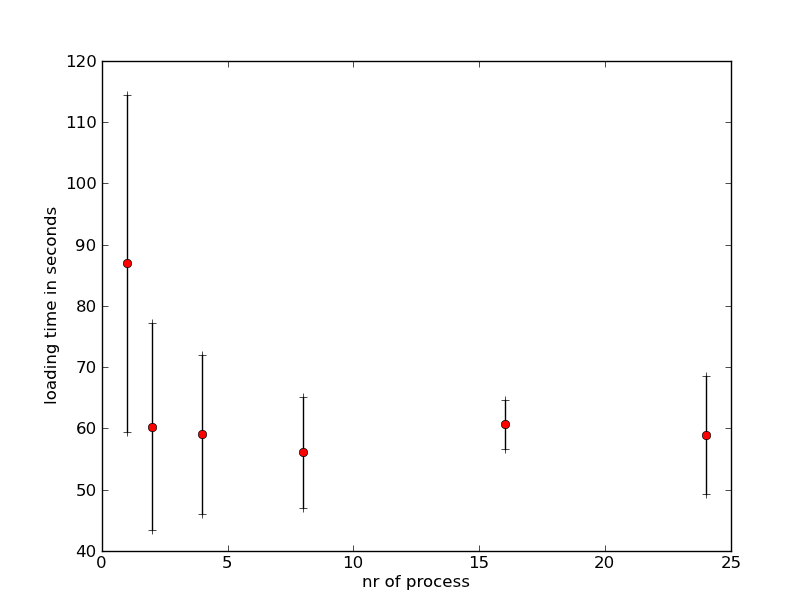
\includegraphics[width=\textwidth]{graphics/openmp17gb/load_time.png}
                \caption{Running time of sequential part, reading the data. 
                         We have average of 10 runns and the standard deviation for each number
                         of processes.}
                \label{fig:openmp_load}
        \end{subfigure}%
         %add desired spacing between images, e. g. ~, \quad, \qquad etc. 
          %(or a blank line to force the subfigure onto a new line)
        \\
        \begin{subfigure}[b]{0.70\textwidth}
                \centering
                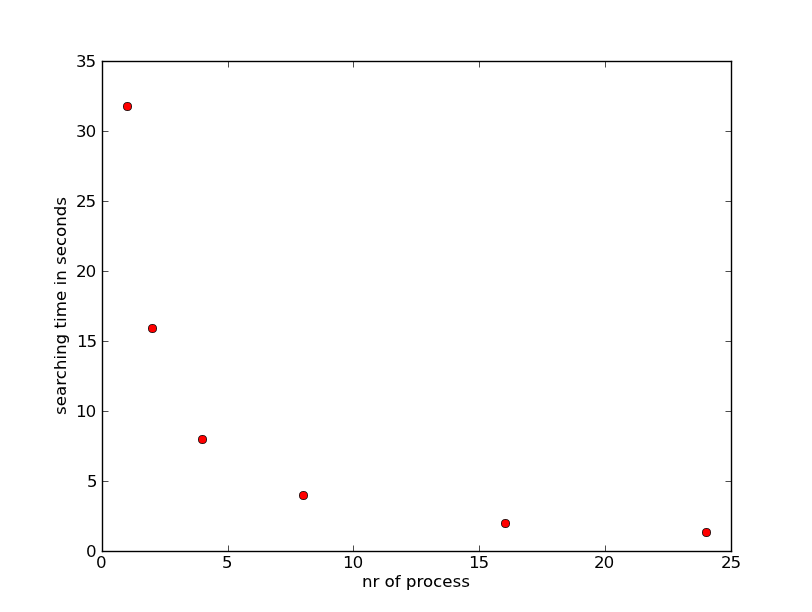
\includegraphics[width=\textwidth]{graphics/openmp17gb/search_time.png}
                \caption{Running time of the parallel part of the code, the actual search. 
                         We have average of 10 runns and the standard deviation for each number
                         of processes (the standard deviation is close to zero so it is hardly 
                         visible)}
                \label{fig:openmp_search}
        \end{subfigure}
        \caption{search time and reading time for the openMP experiment}
\end{figure}


\begin{figure}[htb]
  \centering
  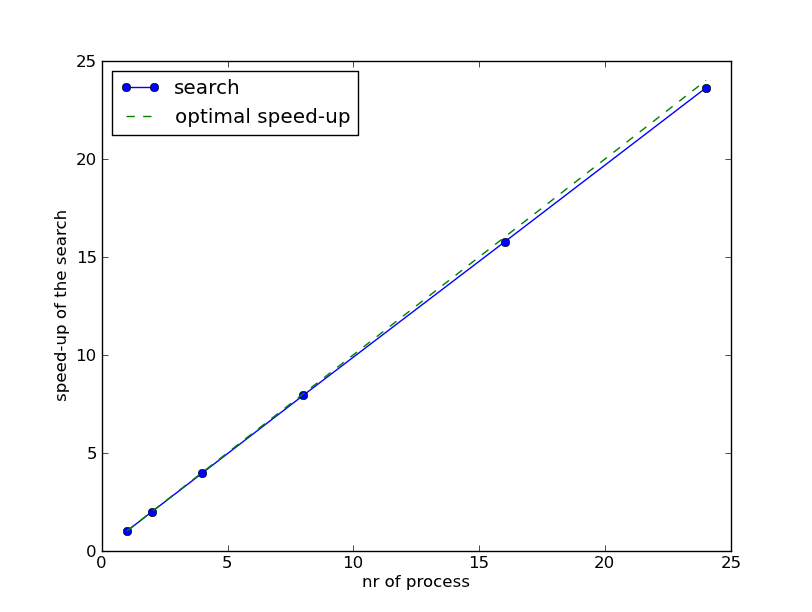
\includegraphics[width=0.7\textwidth]{graphics/openmp17gb/search_speedup.png}
  \caption{Here we see the speed up of the openMP experiemnt.}
  \label{fig:openmp_speedup}
\end{figure}

\begin{figure}[h!t]
        \centering
        \begin{subfigure}[b]{0.70\textwidth}
                \centering
                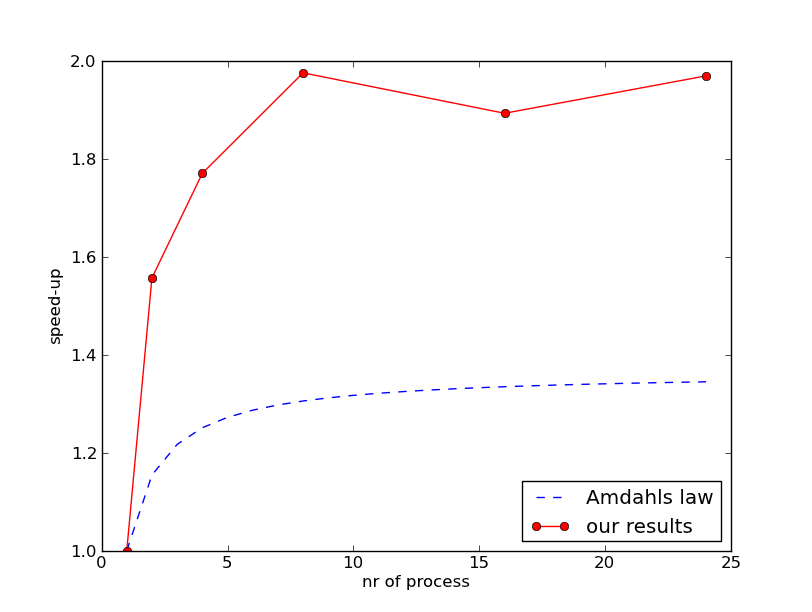
\includegraphics[width=\textwidth]{graphics/openmp17gb/Amdahls_law.png}
                \caption{Here we compare our result with Amdahls law.}
                \label{fig:openmp_amad1}
        \end{subfigure}%
         %add desired spacing between images, e. g. ~, \quad, \qquad etc. 
          %(or a blank line to force the subfigure onto a new line)
        \\
        \begin{subfigure}[b]{0.70\textwidth}
                \centering
                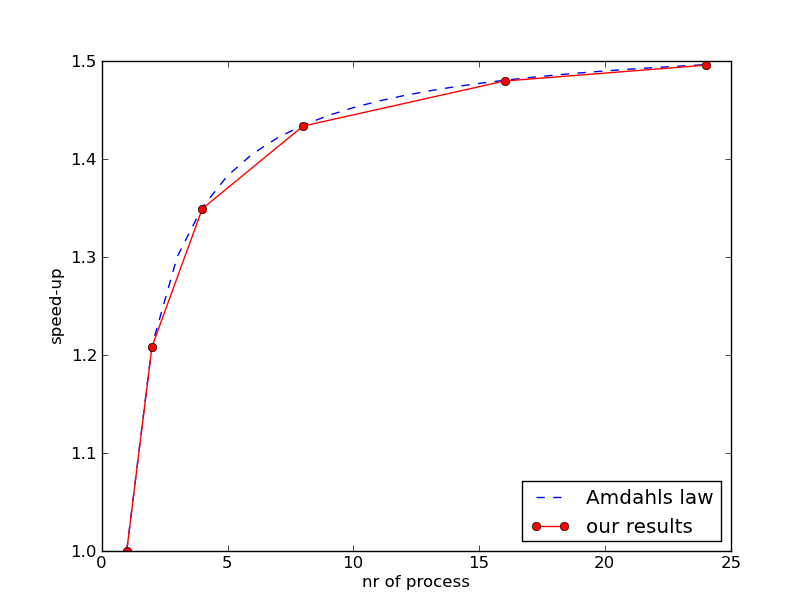
\includegraphics[width=\textwidth]{graphics/openmp17gb/Amdahls_law2.png}
                \caption{Here we compare our results with Amdahls law where we have factored in
                         the diversity in the reading time.}
                \label{fig:openmp_amad2}
        \end{subfigure}
        \caption{Amdahls law for the OpenMP experiment}
\end{figure}


\clearpage
\subsection{MPI with MPI IO}
  For the MPI implementation we did the same experiment as for OpenMP. When we talk about
  reading time and searching time here we mean the reading/searching on the thread that
  took the longest time to read/search.
  With MPI IO we are only able to read int number of bytes, so at maximum $2^{31}-1$ bytes.
  So we could not read our 17gb file on $1,2,4$ threads, and can at minimum read the file if we
  split it up in 8  pieces.  So we need to reduced the 17gb data file down to 2gb to be able to do a full
  speed-up experiment.  We then ran the MPI implementation on the same 17gb data file for 
  $8,16,24$ threads.

  In figure~\ref{fig:mpio2_load} and \ref{fig:mpio2_search} we see the reading time and
  the searching time for the 2gb file.  It seems like the reading time does not depend
  on the number of threads so MPI IO seems to be doing a good job scheduling multiple 
  reads to one file.  If we on the other hand look at figure \ref{fig:mpio_load}, 
  the reading time for the 17gb data file, there seems to be a positive correlation
  between the number of processes and reading time. If we compare the reading time
  for MPI to the reading time for OpenMP we see that the reading time
  for MPI is around 100 seconds and the reading time for OpenMP is around 60 seconds.
  

  In figure \ref{fig:mpio2_speedup} we see the speed-up of the search.  Which is
  close to optimal.  The we can see the speed-up compared to Amdahls law in figure \ref{fig:mpio2_amad1}
  and we fix the reading time as $8$ seconds.

  In figures \ref{fig:mpio2_load} and \ref{fig:mpio_search} we can see the reading time and 
  the searching time for the 17gb data file.  Since we where not able to run the 17gb file 
  on one process we can not really look into the speed-up.  
  It is reasonable to expect a linear speed-up since this part is embarrassingly parallel.
  If we assume linear speed-up then it should take around 24 seconds to run the 17gb file on one process.
  This imaginary speed-up is what we see in figure \ref{fig:mpio_speedup}.

\begin{figure}[h!t]
        \centering
        \begin{subfigure}[b]{0.70\textwidth}
                \centering
                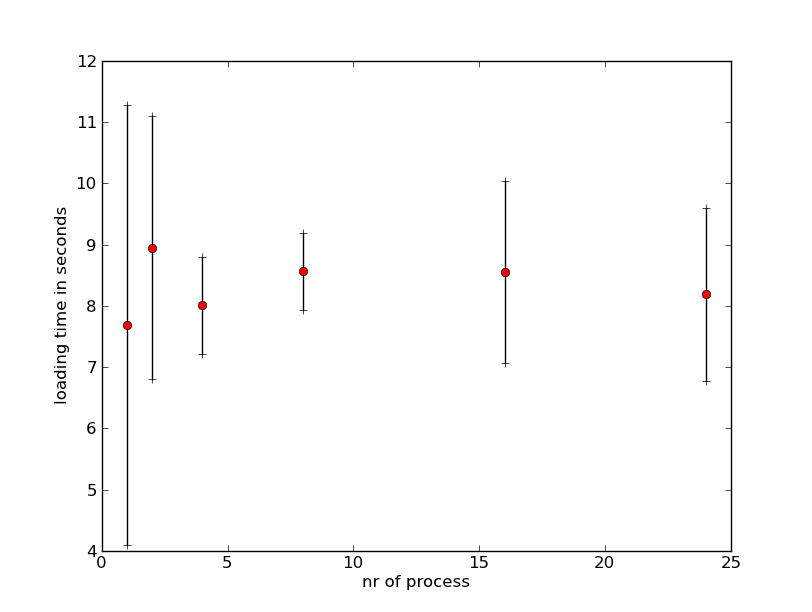
\includegraphics[width=\textwidth]{graphics/mpio2gb_take2/load_time.png}
                \caption{Running time of sequential part, reading the data. 
                         We have average of 10 runns and the standard deviation for each number
                         of processes.}
                \label{fig:mpio2_load}
        \end{subfigure}%
         %add desired spacing between images, e. g. ~, \quad, \qquad etc. 
          %(or a blank line to force the subfigure onto a new line)
        \\
        \begin{subfigure}[b]{0.70\textwidth}
                \centering
                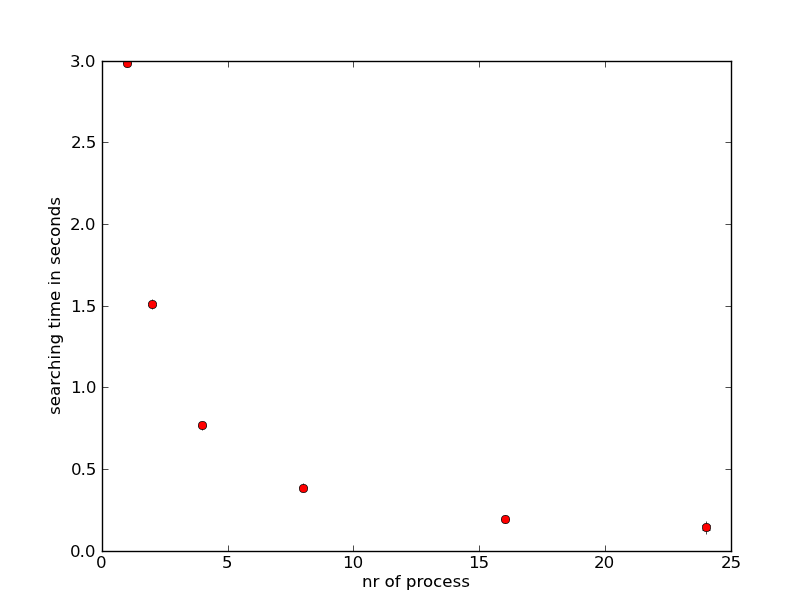
\includegraphics[width=\textwidth]{graphics/mpio2gb_take2/search_time.png}
                \caption{Running time of the parallel part of the code, the actual search. 
                         We have average of 10 runns and the standard deviation for each number
                         of processes (the standard deviation is close to zero so it is hardly 
                         visible)}
                \label{fig:mpio2_search}
        \end{subfigure}
        \caption{search time and reading time for the 2gb data file MPI}
\end{figure}

\begin{figure}[htb]
  \centering
  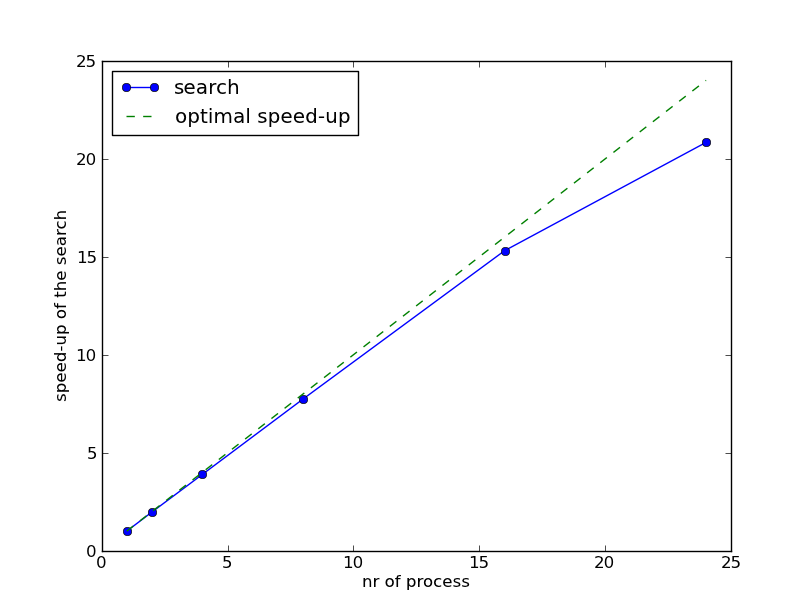
\includegraphics[width=0.7\textwidth]{graphics/mpio2gb_take2/search_speedup.png}
  \caption{Here we see the speed up of the MPI 2gb experiemnt.}
  \label{fig:mpio2_speedup}
\end{figure}

\begin{figure}[h!t]
        \centering
        \begin{subfigure}[b]{0.70\textwidth}
                \centering
                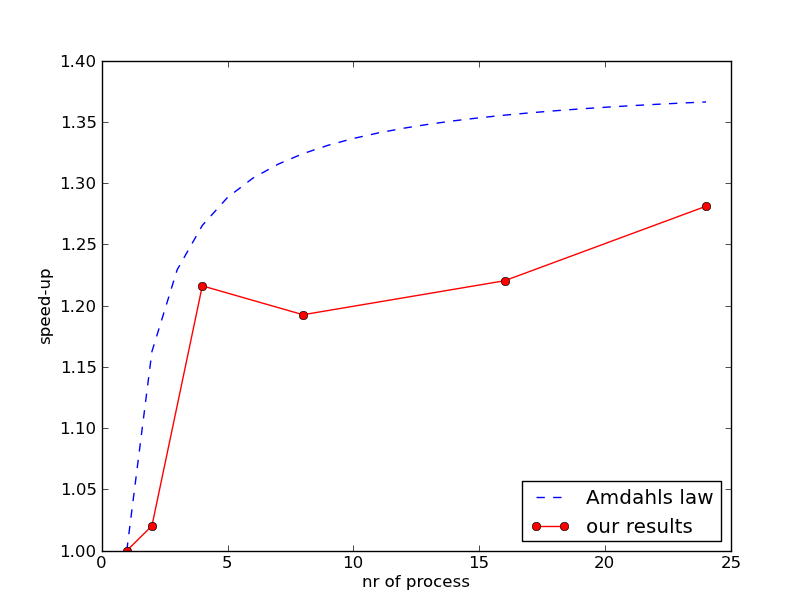
\includegraphics[width=\textwidth]{graphics/mpio2gb_take2/Amdahls_law.png}
                \caption{Here we compare our result with Amdahls law.}
                \label{fig:mpio2_amad1}
        \end{subfigure}%
         %add desired spacing between images, e. g. ~, \quad, \qquad etc. 
          %(or a blank line to force the subfigure onto a new line)
        \\
        \begin{subfigure}[b]{0.70\textwidth}
                \centering
                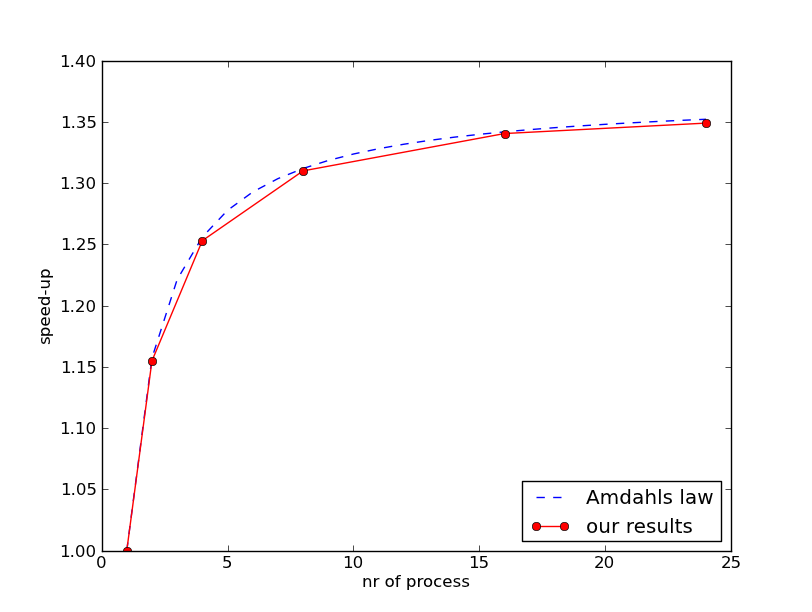
\includegraphics[width=\textwidth]{graphics/mpio2gb_take2/Amdahls_law2.png}
                \caption{Here we compare our results with Amdahls law where we have factored in
                         the diversity in the reading time.}
                \label{fig:mpio2_amad2}
        \end{subfigure}
        \caption{Amdahls law for the 2gb OpenMP experiment.}
\end{figure}

\begin{figure}[h!t]
        \centering
        \begin{subfigure}[b]{0.70\textwidth}
                \centering
                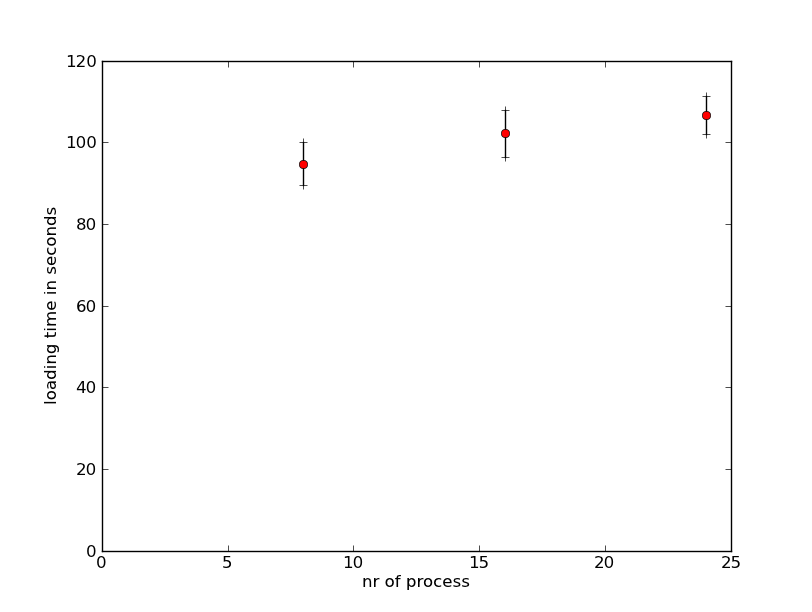
\includegraphics[width=\textwidth]{graphics/mpio17gb/load_time.png}
                \caption{Running time of sequential part, reading the data. 
                         We have average of 10 runns and the standard deviation for each number
                         of processes.}
                \label{fig:mpio_load}
        \end{subfigure}%
         %add desired spacing between images, e. g. ~, \quad, \qquad etc. 
          %(or a blank line to force the subfigure onto a new line)
        \\
        \begin{subfigure}[b]{0.70\textwidth}
                \centering
                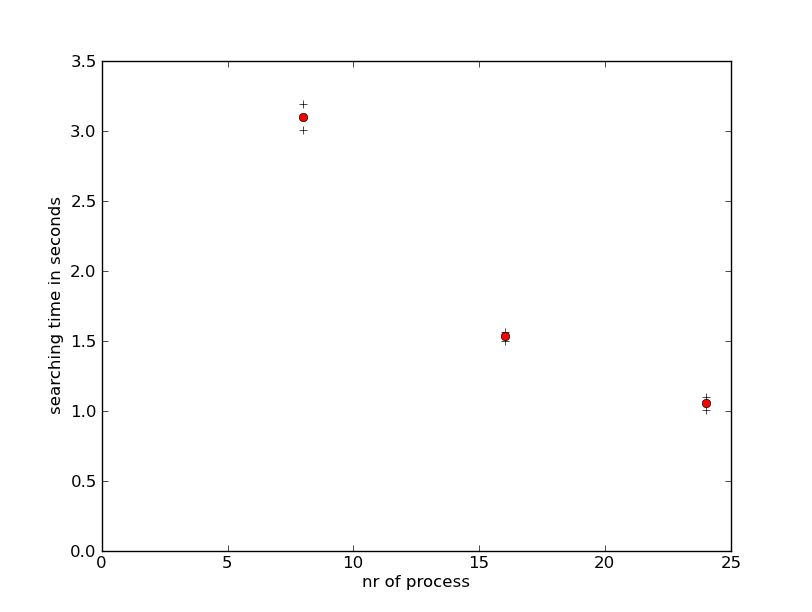
\includegraphics[width=\textwidth]{graphics/mpio17gb/search_time.png}
                \caption{Running time of the parallel part of the code, the actual search. 
                         We have average of 10 runns and the standard deviation for each number
                         of processes (the standard deviation is close to zero so it is hardly 
                         visible)}
                \label{fig:mpio_search}
        \end{subfigure}
        \caption{search time and reading time for the 17gb OpenMP experiment}
\end{figure}

\begin{figure}[htb]
  \centering
  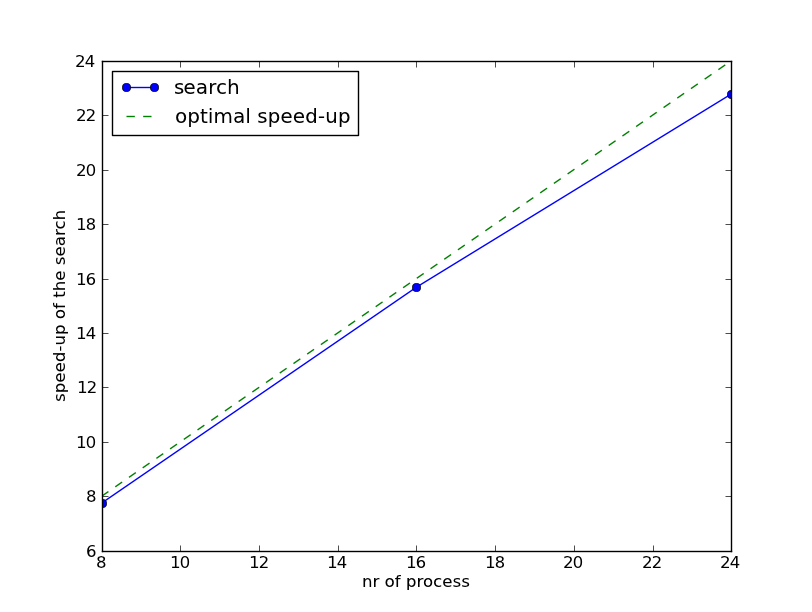
\includegraphics[width=0.7\textwidth]{graphics/mpio17gb/search_speedup.png}
  \caption{Here we see the speed up of the OpenMP 17gb experiment.}
  \label{fig:mpio_speedup}
\end{figure}
\clearpage

\section{MPI single read}
  Finally we like to do some performace analysis with our MPI single read implementation.
  The the mpi scatter function takes only int nr of bytes as offset and data size, so at maximum $2^{31}-1$ bytes.
  So we can only run MPI single read on the 2gb data.

  Only one process reads the data so the reading time should not depend on the number of processes.
  From figure \ref{fig:mpisr_load} we see that the reading time is around 5 for all number of processes.
  In figure \ref{fig:mpisr_search} we see the searching time and the speed up can been seen in 
  figure \ref{fig:mpisr_speedup}. There we see that we get almost no speed-up for 
  1-8 processes but a speed-up about 5 for 16 and 24 processes.  
  This jump could be due latency, that is when we have few processes the network delay
  dominates the gain from using the comminications.
  We are also not getting nearly as good speed up as for the other two implementations.
  We have seen that this problem has a linear speed-up but now when we also have some communiaction
  we are far from getting an optimal speed-up.

  in figure \ref{fig:mpisr_amad1} we see a comparison to our speed-up to Amdahls law.
  Since the reading time does not depend on number of process then it also becomes interesting
  to look at the same graph where the reading time is fixed close to the average reading time.
  In figure \ref{fig:mpisr_amad2} we fix the reading time as $5$ which seems reasonable from
  figure \ref{fig:mpisr_load}.  

\begin{figure}[h!t]
        \centering
        \begin{subfigure}[b]{0.70\textwidth}
                \centering
                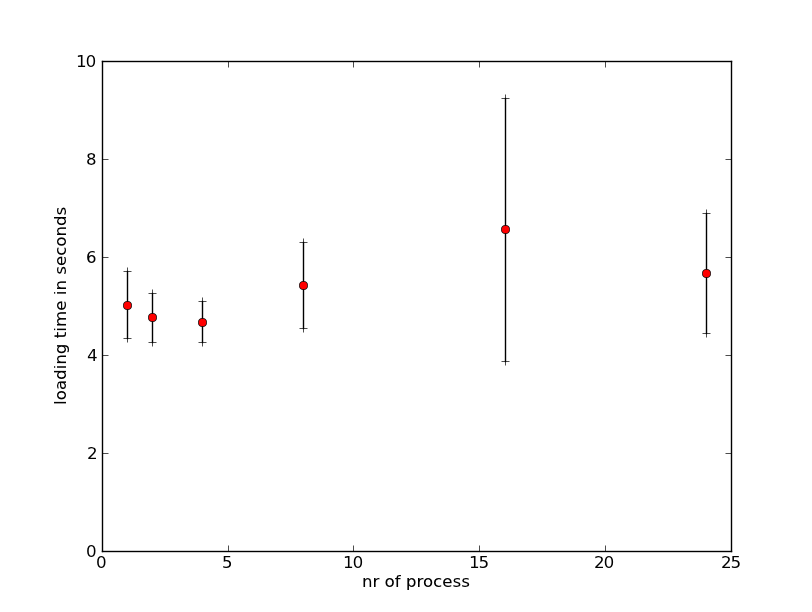
\includegraphics[width=\textwidth]{graphics/mpi2gb_single_reader/load_time.png}
                \caption{Running time of sequential part, reading the data. 
                         We have average of 10 runns and the standard deviation for each number
                         of processes.}
                \label{fig:mpisr_load}
        \end{subfigure}%
         %add desired spacing between images, e. g. ~, \quad, \qquad etc. 
          %(or a blank line to force the subfigure onto a new line)
        \\
        \begin{subfigure}[b]{0.70\textwidth}
                \centering
                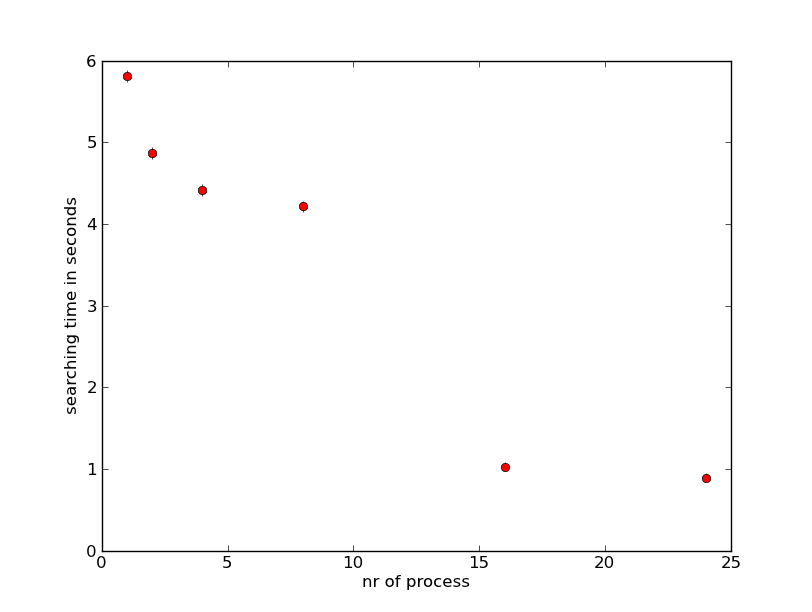
\includegraphics[width=\textwidth]{graphics/mpi2gb_single_reader/search_time.png}
                \caption{Running time of the parallel part of the code, the actual search. 
                         We have average of 10 runns and the standard deviation for each number
                         of processes (the standard deviation is close to zero so it is hardly 
                         visible)}
                \label{fig:mpisr_search}
        \end{subfigure}
        \caption{search time and reading time for the MPI single read experiment}
\end{figure}


\begin{figure}[htb]
  \centering
  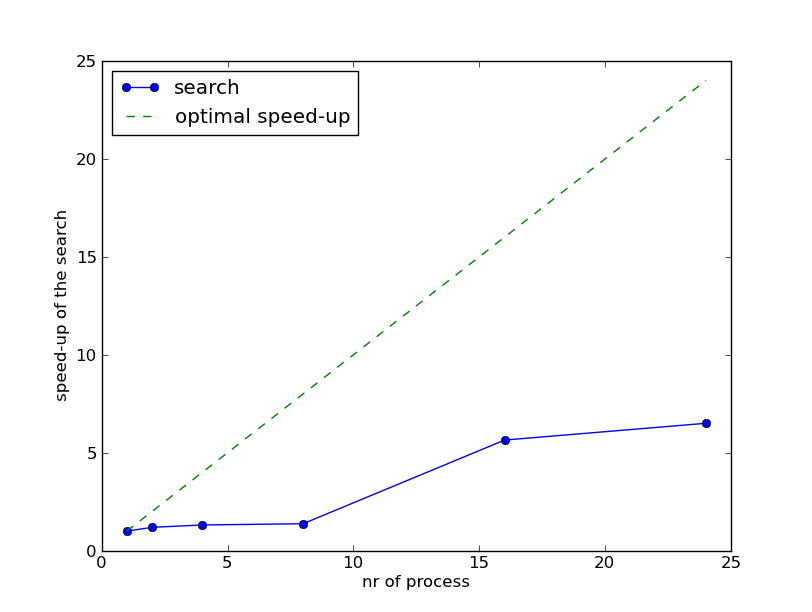
\includegraphics[width=0.7\textwidth]{graphics/mpi2gb_single_reader/search_speedup.png}
  \caption{Here we see the speed up of the MPI single read experiemnt.}
  \label{fig:mpisr_speedup}
\end{figure}

\begin{figure}[h!t]
        \centering
        \begin{subfigure}[b]{0.70\textwidth}
                \centering
                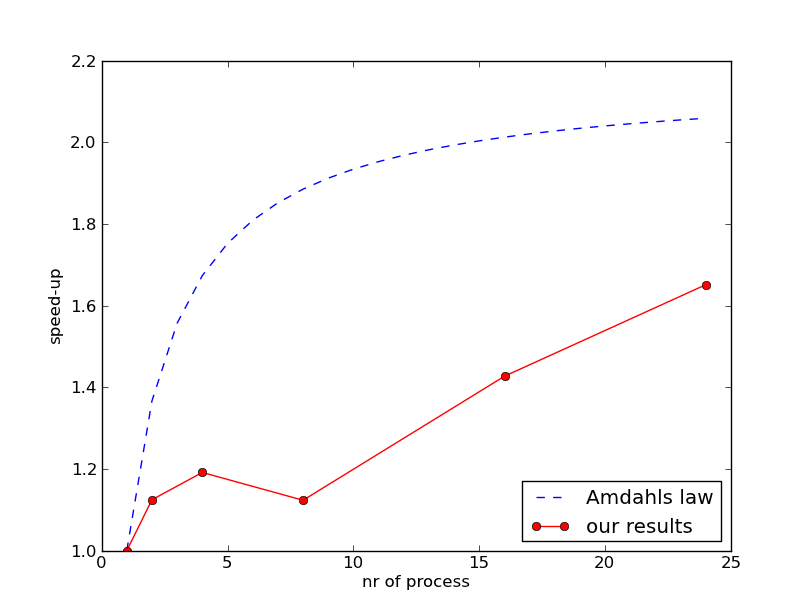
\includegraphics[width=\textwidth]{graphics/mpi2gb_single_reader/Amdahls_law.png}
                \caption{Here we compare our result with Amdahls law.}
                \label{fig:mpisr_amad1}
        \end{subfigure}%
         %add desired spacing between images, e. g. ~, \quad, \qquad etc. 
          %(or a blank line to force the subfigure onto a new line)
        \\
        \begin{subfigure}[b]{0.70\textwidth}
                \centering
                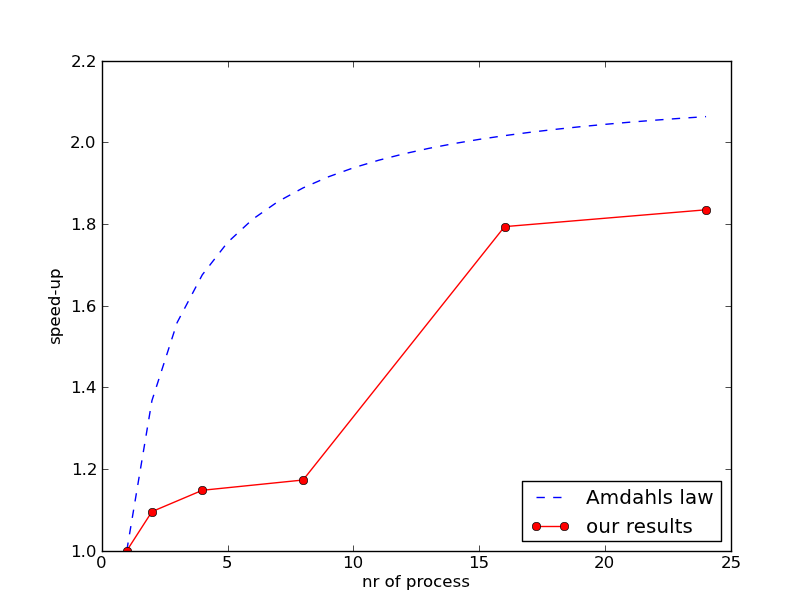
\includegraphics[width=\textwidth]{graphics/mpi2gb_single_reader/Amdahls_law2.png}
                \caption{Here we compare our results with Amdahls law where we have factored in
                         the diversity in the reading time.}
                \label{fig:mpisr_amad2}
        \end{subfigure}
        \caption{Amdahls law for the MPI singal read experiment}
\end{figure}

\clearpage
\section{Conclusions}

Comparing loading times for OpenMP, 
MPI I/O and MPI with single read we see that OpenMP is very consistent in reading a the data file, 
no matter how many processes we use. 
It seems to be comparable with MPI single read, 
as it should since it is basically the same method used there.
We had high hope for MPI I/O for fast parallel file reading, 
but we were surprised by the result. 
On average it seems to be about 50\% slower than the other methods. 
We suspect that the file system used does not support parallel file 
reading and so with more processes there becomes more latency for the file reading process.

For the search part, which we believed to be embarrassingly parallel, 
we got mostly linear speed-up. Both OpenMP and MPI I/O seemed to deliver on that part. 
However when we looked at the MPI with Single read and scattering, 
we seemed to get little speed-up even when we examined only the time after file loading. 
This suggests that the latency in the message interface outweighs the benefit of many 
processes in this case.

We had more problems with MPI than we expected. 
Many of these problems were due to restrictions of counter variables that are usually declared as INT. 
This will however be considered in MPI 3 and this restriction will be fixed. 
There is also supposed to be better support for MPI I/O in MPI 3.

%Skrýtið að stuðningur við stór gögn sé slæmur en það á víst að batna í MPI 3
%$P$ to small.
%Fer frá að vera mjög safaríkt djúsí 
%%%%%%%%%%%%%%%%%%%%%%%%%%%%%%%%%%%%%%%%%%
%%%%%%%%%%%%%%%%%%%%%%%%%%%%%%%%%%%%%%%%%%
%%%%%%
%%%%%%  Appendix  
%%%%%%
\appendix
\section{Code}
%  \subsection{serial code}
%    \lstinputlisting[language=C]{../src/search_serial.c}
  \subsection{OpenMP}
    \lstinputlisting[language=C]{../src/search_openmp.c}   
  \subsection{MPI whit MPI IO}
    \lstinputlisting[language=C]{../src/search_mpio.c} 
    \subsection{MPI single read}
    \lstinputlisting[language=C]{../src/search_mpi_single_reader.c}
\end{document}          
